% AAAI-26 投稿模板（官方 AuthorKit26 的 aaai2026.sty / aaai2026.bst 已随模板附带）
% 双盲投稿用 [submission]；录用后改为 \usepackage{aaai2026} 并去掉 \nocopyright 相关限制
\documentclass[letterpaper]{article}
\usepackage[submission]{aaai2026}
\usepackage{times}
\usepackage{helvet}
\usepackage{courier}
\usepackage[hyphens]{url}
\usepackage{graphicx}
\urlstyle{rm}
\def\UrlFont{\rm}
\usepackage{natbib}
\usepackage{caption}
\frenchspacing
\setlength{\pdfpagewidth}{8.5in}
\setlength{\pdfpageheight}{11in}

% 公式、三线表与合并单元格
\usepackage{amsmath}
\usepackage{amssymb}
\usepackage{booktabs}
\usepackage{multirow}

\pdfinfo{
/TemplateVersion (2026.1)
}

\setcounter{secnumdepth}{2}

\begin{document}

\title{A Compact AAAI-26 Format Example with Figures and Tables}

\author{Anonymous Submission\\
Paper ID: 0000}

\maketitle

\begin{abstract}
This sample demonstrates the AAAI-26 two-column layout produced by
\texttt{aaai2026.sty}: an included bitmap figure, a \texttt{booktabs}
table, a merged-cell table, a numbered equation and AAAI-formatted
references. Replace the content with your own manuscript.
\end{abstract}

\section{Introduction}
AAAI papers are limited to seven pages of technical content plus
references. The \texttt{aaai2026.sty} file already sets the
bibliography style, so no \verb|\bibliographystyle| command is needed.
Note that \texttt{hyperref} is not allowed with this style.
Related work builds on the Transformer~\cite{vaswani2017attention} and
residual networks~\cite{he2016deep}.

\section{Figures}
Figure~\ref{fig:curve} is inserted at column width with
\verb|\includegraphics|. Crop whitespace in your own figures and keep
labels legible at 100\%.

\begin{figure}[t]
  \centering
  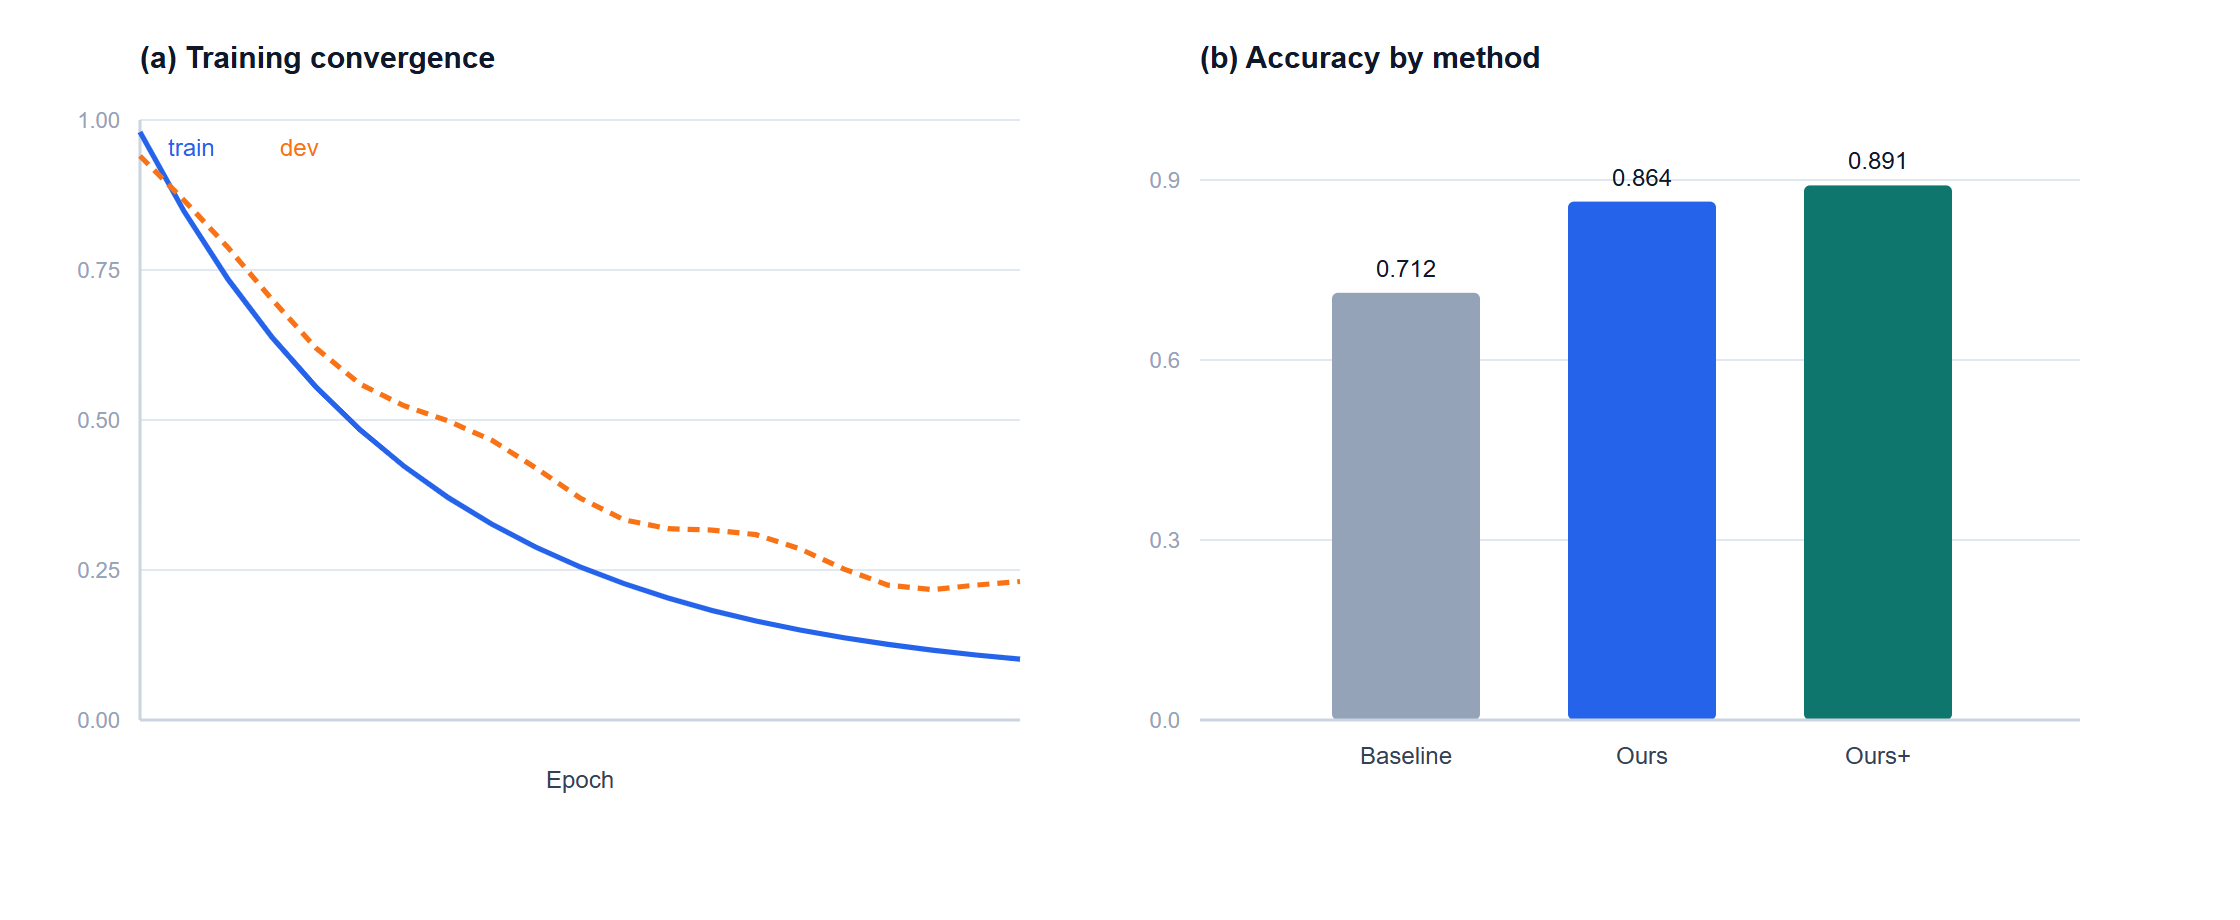
\includegraphics[width=\columnwidth]{figure.png}
  \caption{Training convergence and accuracy comparison.}
  \label{fig:curve}
\end{figure}

\section{Tables}
Table~\ref{tab:main} uses \texttt{booktabs} rules,
Table~\ref{tab:merged} merges header cells with \texttt{multirow} and
\texttt{cmidrule}.

\begin{table}[t]
  \caption{Accuracy of different methods.}
  \label{tab:main}
  \centering
  \begin{tabular}{lcc}
    \toprule
    Method & Dev & Test \\
    \midrule
    Baseline & 0.712 & 0.705 \\
    Ours     & 0.864 & 0.871 \\
    Ours+    & \textbf{0.891} & \textbf{0.883} \\
    \bottomrule
  \end{tabular}
\end{table}

\begin{table}[t]
  \caption{Backbone comparison with merged header cells.}
  \label{tab:merged}
  \centering
  \begin{tabular}{llc}
    \toprule
    \multirow{2}{*}{Model} & \multirow{2}{*}{Backbone} & Accuracy \\
    \cmidrule(l){3-3}
     & & (test) \\
    \midrule
    Ours  & ViT-B & 0.871 \\
    Ours+ & ViT-L & 0.883 \\
    \bottomrule
  \end{tabular}
\end{table}

\section{Equations}
Equation~\eqref{eq:gauss} shows display math in the AAAI column width.

\begin{equation}
  f(x)=\frac{1}{\sqrt{2\pi}\,\sigma}
  \exp\!\left(-\frac{(x-\mu)^2}{2\sigma^2}\right)
  \label{eq:gauss}
\end{equation}

\section{Conclusion}
The style file and bibliography style ship with this template, so the
project compiles without any extra download.

\bibliography{refs}

\end{document}
